%
% tikztemplate.tex -- template for standalon tikz images
%
% (c) 2021 Prof Dr Andreas Müller, OST Ostschweizer Fachhochschule
%
\documentclass[tikz]{standalone}
\usepackage{amsmath}
\usepackage{times}
\usepackage{txfonts}
\usepackage{pgfplots}
\usepackage{csvsimple}
\usetikzlibrary{arrows,intersections,math}
\begin{document}
\def\skala{1}
\begin{tikzpicture}[>=latex,thick,scale=\skala]
\clip (-5.8,-3.65) rectangle (4.3,3.65);

\node at (-3.3,0) {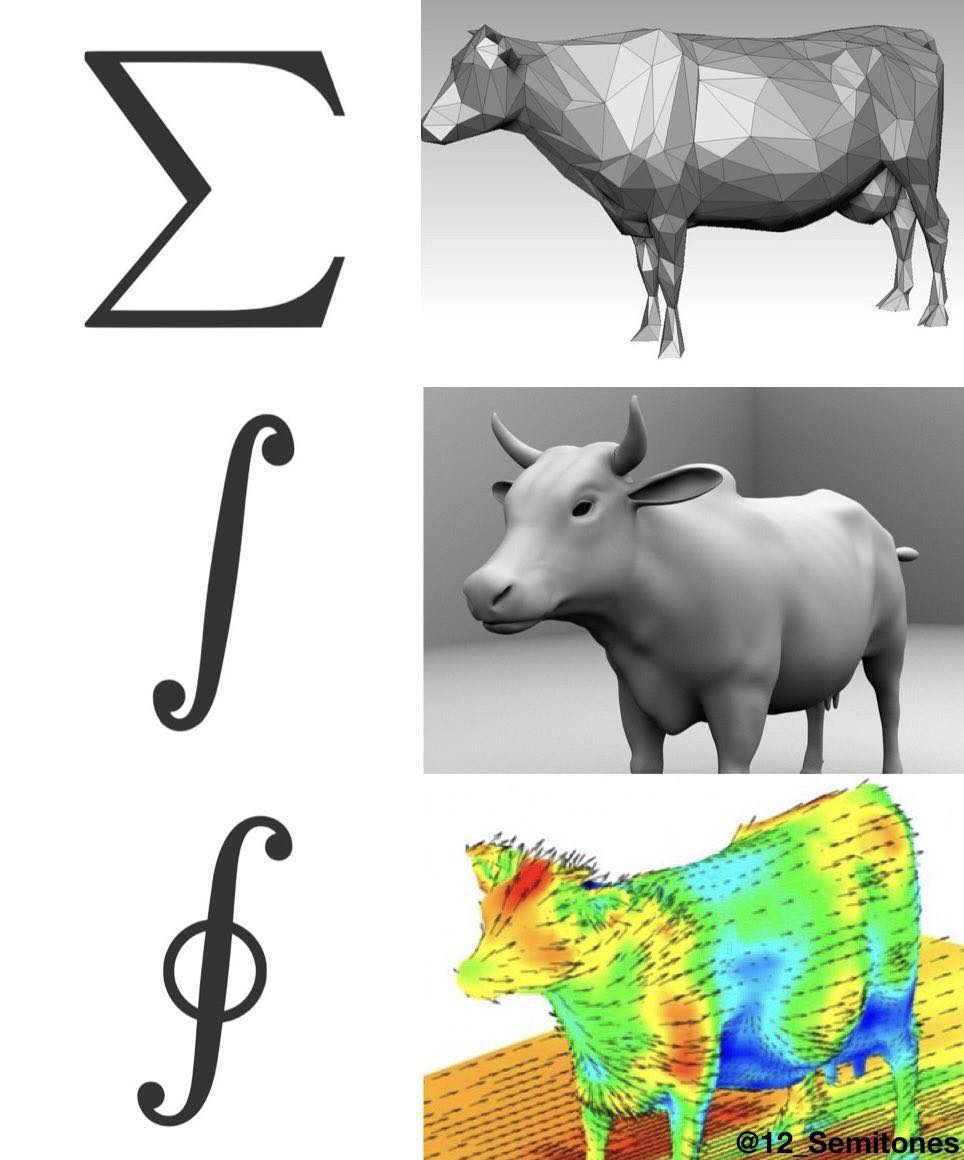
\includegraphics[width=6cm]{kuh.png}};
\node at (3.3,0) {\begin{minipage}{6cm}
\end{minipage}};
\node at (0.9,2.5) [right]
	{$\displaystyle V = \sum_{i=1}^N \operatorname{vol}(S_i)$};
\node at (0.9,0) [right]
	{$\displaystyle V = \underset{}K{\int\!\!\!\int\!\!\!\int} 1\, dx\,dy\,dz$};
\node at (0.9,-2.5) [right]
	{$\displaystyle F = \oint_{\partial K} \omega$};

\end{tikzpicture}
\end{document}

